\subsection{Unlocking the Secrets of Series Capacitors in Gamma Matches!}

\begin{tcolorbox}[colback=gray!10, colframe=black, title=E9E04]
What is the purpose of the series capacitor in a gamma match? 
\begin{enumerate}[label=\Alph*)]
    \item A: To provide DC isolation between the feed line and the antenna
    \item \textbf{B: To cancel unwanted inductive reactance}
    \item C: To provide a rejection notch that prevents the radiation of harmonics
    \item D: To transform the antenna impedance to a higher value
\end{enumerate} \end{tcolorbox}

\subsubsection{Related Concepts}

In radio communication, gamma matches are employed to improve the impedance matching between an antenna and a feed line. This is critical for maximizing power transfer and reducing signal loss. The gamma match consists of a spar or a conductor element that provides the necessary impedance transformation. The series capacitor included in this configuration plays a significant role in managing the reactive components of the antenna's impedance, especially the unwanted inductance.

\subsubsection{Understanding Inductive Reactance}

Inductive reactance ($X_L$) is a measure of how much an inductor resists the change in current flow in an alternating current (AC) circuit. It can be calculated using the formula:

\[
X_L = 2 \pi f L
\]

where:
- \(f\) is the frequency of the signal in hertz (Hz),
- \(L\) is the inductance in henries (H).

When we have unwanted inductive reactance in the circuit, it can potentially lead to a mismatch in impedance, which can cause reflected power and reduced efficiency. 

The purpose of the series capacitor in the gamma match is to introduce a capacitive reactance ($X_C$) that can counteract the inductive reactance. The capacitive reactance can be calculated using the formula:

\[
X_C = \frac{1}{2 \pi f C}
\]

where \(C\) is the capacitance in farads (F).

The goal of using a capacitor is to make the total reactance zero:

\[
X_L + X_C = 0 \implies X_C = -X_L
\]

This means that by selecting a capacitor with an appropriate value, we can cancel out the unwanted inductive reactance, thereby allowing efficient energy transfer.

\subsubsection{Conceptual Diagram}

Below is a simple illustration of a gamma match configuration showing the series capacitor and its connection to the antenna:

\begin{center}
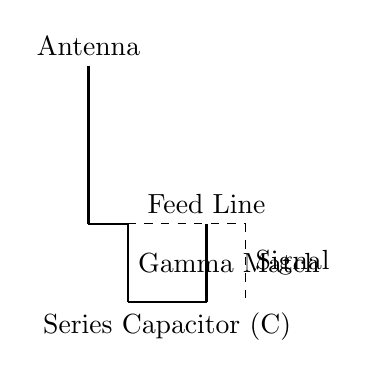
\begin{tikzpicture}
    % Draw the antenna
    \draw[thick] (0,0) -- (0,2) node[above] {Antenna};
    
    % Draw the gamma match
    \draw[thick] (0.5,0) -- (0.5,-1) node[midway, right] {Gamma Match};
    \draw[thick] (0,0) -- (0.5,0);
    
    % Draw the series capacitor
    \draw[thick] (0.5,-1) -- (1.5,-1) node[midway, below] {Series Capacitor (C)};
    \draw[thick] (1.5,-1) -- (1.5,0) node[above] {Feed Line};
    
    % Draw connections
    \draw[dashed] (2,0) -- (2,-1) node[midway, right] {Signal};
    \draw[dashed] (0.5,0) -- (2,0);
\end{tikzpicture}
\end{center}

In conclusion, the series capacitor in a gamma match is essential for cancelling unwanted inductive reactance, thus ensuring optimal performance of the communication system.
